\documentclass[12pt, a4paper,leqno]{report}
\usepackage[utf8]{inputenc}
\usepackage{amssymb}
\usepackage{amsthm}
\usepackage{amssymb, amsmath}
\usepackage[bookmarksnumbered=true,bookmarksopen=true, pdfborder={0 0 0}]{hyperref}
\hypersetup{pdfborder={0 0 0}}
\usepackage{graphicx}

\newenvironment{solution}{\paragraph{\normalfont{\textit{Solution}}.}}{\hfill\null$\square$}

\newtheoremstyle{normal}{}{}{}{}{\normalfont\bfseries}{.}{ }{}

\newtheorem{definition}{Definition}[chapter]
\newtheorem{lemma}{Lemma}[chapter]
\theoremstyle{normal}
\newtheorem{exercise}{Exercise}[chapter]
\theoremstyle{normal}
\newtheorem{example}{Example}[chapter]

\def\expect{\mathbb{E}}

\title{Naïve Decision Making}
\author{Dimitar Vouldjeff}

\begin{document}
	\maketitle
	\tableofcontents
	
	\chapter{Introduction}
	
	\chapter{Probability}
	\section{Short probability theory}
	In this section we set out some rules which we call 'probability theory'. It is the separate job of statisticians to attempt to apply this theory to the real world and that of philosophers to worry why such an application can be made.
	
	We start with a non-empty finite set $\Omega$ called the \textit{probability space}. For example a horse race with $n$ horses:
	\[ \Omega = \lbrace \omega_1, \omega_2, \dots\omega_n \rbrace \]
	with $\omega_j$ the point corresponding to the $j$th horse winning.
	Also there is a function $p : \Omega \rightarrow \mathbb{R}$ such that $p(\omega)\geq 1$ for every $\omega\in\Omega$ and:
	\[ \sum\limits_{\omega\in\Omega} p(\omega) = 1. \]
	With other words the sum of all the points` probabilities within a single space must be $1$.
	
	Let $A$ be a subset of $\Omega$ then:
	\[ Pr(A) = \sum\limits_{\omega\in A} p(\omega) \]
	We call $Pr(A)$ the probability of event $A$ and 
	\[ Pr(A) = \frac{\text{the number of ways an event can occur}}{\text{the number of all the events}} \]\\
	\begin{list}{$\bullet$}{\textbf{Properties:}}
		\item For every event $A$, $1 \leq Pr(A) \leq 0$.
		\item If $A$ and $B$ are disjointed events, then $Pr(A\cup B) = Pr(A) + Pr(B)$.
	\end{list}
	
	\section{Combinatorics}
	Probability becomes much easier to understand when consider some basic models.
	One of them is how for example a deck of $n$ cards can be dealt. The first card may be any of the $n$ cards, the second any of the remaining $n - 1$ cards and so on. Thus there are:
	\[ n! = n(n - 1)(n - 2)\dots 1 \]
	ways of dealing the cars. This is called permutation of $n$ elements. And by definition $0! = 1$.\\
	
	\noindent\textbf{Rule of sum:} If $A$ can be chosen in $n$ ways and $B$ in $m$ then any of the elements $M$ or $N$ can be chosen in $n+m$ ways.\\
	
	\noindent\textbf{Rule of product:} If $A$ can be chosen in $n$ ways and in every choice of $A$ $B$ can be chosen in $m$ ways then $(A, B)$ can be chosen in $nm$ ways.\\
	
	\begin{example}
		Find in how many different ways can five students sit on bench, having in mind that two of them want to be together?
		\begin{solution}
			Consider the two students who want to be together as one. Then we have $4!$ different ways, but the couple can also swap their places, thus the final number is
			\[ 2P_4 = 48. \]  
		\end{solution}
	\end{example}
		
	Assuming the probability of all the deals to be the same, we are obtaining a probability space $\Omega$ with $n!$ elements such that for every $\omega\in\Omega$:
	\[ Pr(\lbrace\omega\rbrace) = \frac{1}{n!} \]
	
	But what if we want to know how many 5 cards poker hands are there from a 52 cards deck?
	
	\begin{lemma}
		If a set has $n$ elements the number of $k$ distinct combination is:
		\[ \binom{n}{k} = \frac{n!}{k!(n-k)!} \]
		\begin{proof}
			We can also use $\dbinom{n}{k}$ as the coefficient of $x^ny^{n-k}$ in $(x+y)^n$, or in other words
			\[ (x+y)^n = \binom{n}{0}x^n + \binom{n}{1}x^{n-1}y + \binom{n}{2}x^{n-2}y^2 +\dots + \binom{n}{n}y^n. \]
			Because of that fact $\binom{n}{k}$ is called a \textit{binomial coefficient}.
		\end{proof}
	\end{lemma}
	
	\begin{exercise}
		 Let we have an $m$ sided die with $b$ of them coloured blue and the rest - red. If we throw the die $n$ times the probability of any sequence with exactly $r$ blue sides is $p^r(1-p)^{n-r}$ where $p = \dfrac{b}{m}$.
		 If $A_r$ is this event, then
		 \[ Pr(A_r) = \binom{n}{r}p^r(1-p)^{n-r}. \]
		 \begin{solution}
		 	Each blue face can arise in $b$ ways and each red in $m-b$ and
		 	\[ \underbrace{b\times b\times\dots\times b}_{\mbox{r times}}\times \underbrace{(m-b)\times (m-b)\times\dots\times (m-b)}_{\mbox{n-r times}} = b^r(m-b)^{n-r} \]
		 	We know that there are $\dbinom{n}{r}$ different ways of arranging the aforementioned sequence, so
		 	\[ Pr(A_r) = \binom{n}{r}p^r(1-p)^{n-r} \]
		 	as stated.
		 \end{solution}
	\end{exercise}
	
		\section{Conditional probability}	
	When in a random experiment the event $B$ is known to have occurred, the possible outcomes of the experiment are reduced to B, and hence the probability of the occurrence of $A$ is changed from the unconditional probability into the conditional probability given $B$.
	
	Let $\Omega$ be a probability space with associated probability $Pr$. If the event $B$ occurred, $A,B\in\Omega$ and $Pr(B) > 0$
	\[ Pr(A|B) = \frac{Pr(A\cap B)}{Pr(B)} \] 
	
	\begin{example}
		What is the probability that the total of two dice will be greater than 8, given the first die is a 6?
		\begin{solution}
			Let $A, B\in\Omega$, $B$ is the event the first die is a 6 and $A$ is the event the total is greater than 8.
			$Pr(B) = \frac{1}{6}$ and $Pr(A) = \frac{4}{6}$, thus
			\[ Pr(A|B) = \frac{Pr(A\cap B)}{Pr(B)} = \frac{\frac{1}{6}.\frac{4}{6}}{\frac{1}{6}} = \frac{2}{3} \]
		\end{solution}
	\end{example}
	
	\section{Independent events}
	In probability theory, to say that two events are \textit{independent} intuitively means that the occurrence of one event makes it neither more nor less probable that the other occurs.
	Let $\Omega$ be a probability space with associated probability $Pr$.
	We say that two events $A, B\in\Omega$ are independent if
	\[ Pr(A\cap B) = Pr(A)Pr(B). \]
	
	\begin{example}
		A die is tossed twice. Find the probability of getting a 4 or 5 on the first toss and a 1, 2, or 3 in the second toss.
		\begin{solution}
			Let $A, B\in\Omega$ with probability $Ar$ and $A$ is the event of the first toss, $B$ of the second. Thus $Pr(A) = \frac{1}{3}$ and $Pr(B) = \frac{1}{2}$. The two events are obviously independent, so
			\[ Pr(A\cap B) = Pr(A)Pr(B) = \frac{1}{3}.\frac{1}{2} = \frac{1}{6}. \] 
		\end{solution}
	\end{example}	
	
	\section{Random variables}
	In probability theory and statistics a \textit{random variable} is function which maps events of outcomes to values.
	There are two types of random variables - \textit{discrete} and \textit{continuous}. A discrete random variable maps outcomes to values of a countable set (e.g. integers), while continuous maps to values of uncountable sets (e.g. real numbers).
	
	\begin{example}
		\label{ex:die_x}
		A discrete random variable can be used to describe the process of rolling a die and the possible outcomes. Take the set $\Omega = \lbrace 1, 2, 3, 4, 5, 6\rbrace$ as the state space, defining the random variable $X$ equal to the number rolled.
		In this case
		\[ X(\omega) = \begin{cases}
			1, & \text{if a 1 is rolled} ,\\
			2, & \text{if a 2 is rolled} ,\\
			3, & \text{if a 3 is rolled} ,\\
			4, & \text{if a 4 is rolled} ,\\
			5, & \text{if a 5 is rolled} ,\\
			6, & \text{if a 6 is rolled} .
		\end{cases} \]
	\end{example}
	
	\begin{example}
		The following random variable is continuous
		\[ X = \text{the exact amount of rain tomorrow}. \]
	\end{example}
	
	\noindent Every random variable has its \textit{expectation} (or \textit{expected value}) written $\expect X$ or $\mu$ and
	\[ \expect X = \sum\limits_{\omega\in \Omega} p(\omega) X(\omega). \]
	For example the expectation in Example \ref{ex:die_x} is
	\[ \expect X = 1.\frac{1}{6} + 2.\frac{1}{6} + 3.\frac{1}{6} + 4.\frac{1}{6} + 5.\frac{1}{6} + 6.\frac{1}{6} = 3,5 . \]	
	
	\section{Law of large numbers}
	The \textit{Law of large numbers} is one of the most intuitive laws in mathematics and probability.
	Let $X$ is a random variable and $\expect X = \mu$ the expected value.
	\[ \overline{X}_n = \frac{x_1 + x_2 + \dots + x_n}{n} \]
	is called \textit{sample mean} and the law says that
	\[ \overline{X}_n \to \mu \ \ \ \text{when} \ \ \ n\to\infty \]
	
	And Because the law of large numbers is so applicable it is very often misunderstood. Let us consider the following scenario. You are tossing a coin with a random variable $X$ (1 for head, 0 for trail) and thus the expected value $\mu = 0.5$. After a finite number of tosses (e.g. 10) the sample mean $\overline{X}_n = 0,8$. In such situations people tend to thing that the Gods of probability will somehow make the next few tosses to be trails in order to compensate (this perception is called \textit{the Gambler`s fallacy}). But that is usually not the case. What the law of large numbers says is "I do not care when the sample mean will converge to the expected value! You have a infinite number of tosses."
	\begin{figure}[h!]
		\caption{An illustration of coin tossing.}
		\centering
			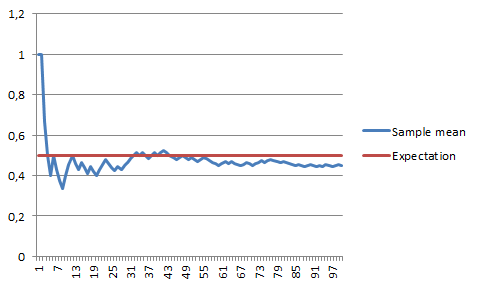
\includegraphics[width=12cm]{graphic.png}
	\end{figure}	
	
	\section{Kelly criterion}
	The \textit{Kelly Criterion} is used to determine what amount of your money to bet when you know the odds. In most gambling and investing the Kelly strategy will do better than any essentially different strategy long term. This simple formula stands behind the success of world known investors like Worren Buffett.
	
	Imagine you are betting on a coin flip. On heads if you bet 1\$ you will get 2\$ and on trails - you loose the dollar. Then $\mu = 0,5$ or $\mu = 50\%$, so how could you loose money in such a case? The answer is very simple - by betting to much and here Kelly comes to the rescue!
	\[ K = \frac{pb - (1 - p)}{b} \]
	where $K$ is the optimal percentage you should bet, $p$ is the odds you will win the bet, $b$ is the payout (in our case 2) and $1-p$ represents the odds you will loose. Let us calculate the best betting percentage
	\[ K = \frac{0,5\times 2 - (1-0,5)}{2} = 0,25 \] 
	If you bet more than 25\% your profit will grow, but slower, and if you bet more than 50\% (twice as much) you will experience \textit{over-betting}.
	\begin{figure}[h!]
		\caption{An illustration of the two main ways of betting.}
		\centering
			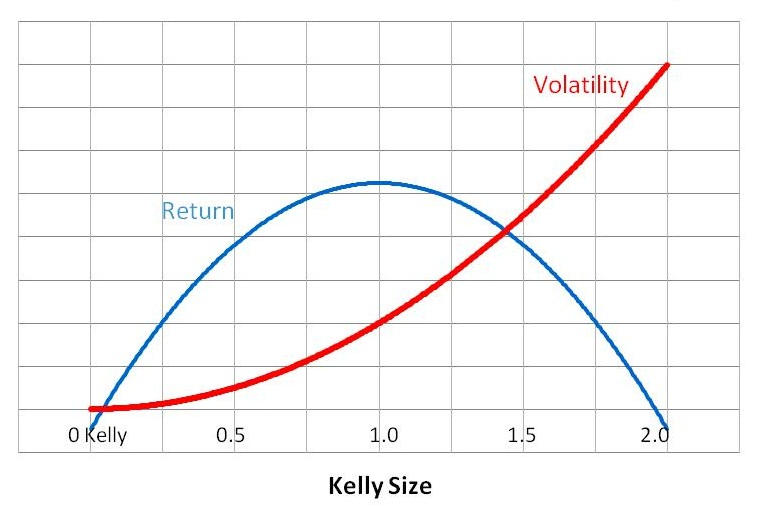
\includegraphics[width=12cm]{kelly.jpg}
	\end{figure}
	
	\chapter{Statistics}
	\section{Probability distribution function}
	A mathematical function can be used to model the frequencies and probabilities of occurrences over time. A \textit{discrete probability distribution function} associates each possible value of a discrete random variable with it`s probability. The probabilities of a continuous random variable are modelled using \textit{continuous distribution functions}, also known as \textit{probability density functions}.
	
	\subsection{Binomial distribution}
	In order to understand what a \textit{binomial distribution} is, first you have to be familiar with the \textit{binomial experiment}. A binomial experiment (or \textit{Bernoulli trial}) is a statistical experiment that has the following properties:
	\begin{itemize}
		\item The experiment consists of $n$ repeated trials.
		\item Each of the trials can result in success or failure.
		\item The probability on success is the same for every trials.
		\item The trials are independent.
	\end{itemize}
	Another important thing to know is that a \textit{binomial random variable} represents the number of successes in $n$ repeated trials of a binomial experiment. The \textit{probability distribution} of a binomial random variable is called a \textit{binomial distribution}.

	\begin{example}
		You are shooting at a target and the possibility of hitting it is $0,6$ for example. We have a binomial random variable 
		\[ X = \text{the number of successful shootings in } n = 5 \text{ trials}. \] 
		Make a binomial distribution graph.
		\begin{solution}
			In order to make the graph we first need to know the probability for each of the random variable`s values.		
			\[\begin{split}
  				Pr(X = 0) = & \textit{number of such cases } \times \textit{ probability of each case} \\
   				= & \binom{n}{0} \times \textit{ probability of success}^0 \times \textit{ probability of failure}^{n - 0} \\
   				= & 1\times 1\times (1-0,6)^5 \\
   				= & 0,0102 \\
   				\\
  				Pr(X = 1) = & \textit{number of such cases } \times \textit{ probability of each case} \\
   				= & \binom{n}{1} \times \textit{ probability of success}^1 \times \textit{ probability of failure}^{n - 1} \\
   				= & 5\times 0,6\times (1-0,6)^4 \\
   				= & 0,0768 \\
   				\\
  				Pr(X = 2) = & \binom{n}{2} \times 0,6^2 \times 0,4^3 \\
   				= & 0,2304 \\
   				\\
  				Pr(X = 3) = & \binom{n}{3} \times 0,6^3 \times 0,4^2 \\
   				= & 0,3456 \\
   				\\
  				Pr(X = 4) = & \binom{n}{4} \times 0,6^4 \times 0,4^1 \\
   				= & 0,2592 \\ 
   				\\
  				Pr(X = 5) = & \binom{n}{5} \times 0,6^5 \times 0,4^0 \\
   				= & 0,0777
			\end{split}\]
			And then we make the graph
			\begin{figure}[h!]
				\caption{Binomial distribution graph.}
				\centering
					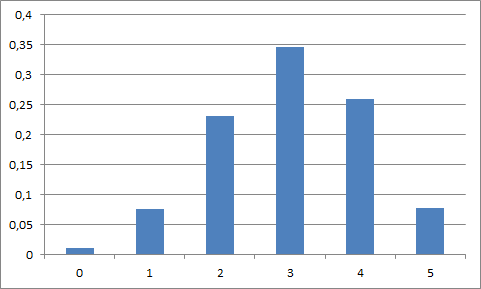
\includegraphics[width=12cm]{binomial_graph.png}
			\end{figure}			
			
		\end{solution}
	\end{example}	
	
	\subsection{Normal distribution}	
	
	
	
	\chapter{Conclusion}


\end{document}